\documentclass[tikz,border=2pt]{standalone}
\usetikzlibrary{arrows.meta,positioning,calc,shapes.geometric}
\usepackage{fontspec}
\setmainfont{TeX Gyre Termes}
\setsansfont{Roboto}
\begin{document}
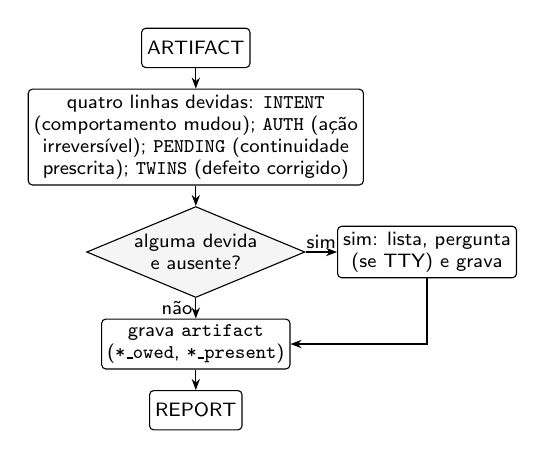
\begin{tikzpicture}[
  font=\sffamily\scriptsize, >={Stealth[length=4pt]},
  proc/.style={draw, thin, rounded corners=1.5pt, align=center, fill=white, minimum height=0.5cm, inner sep=2pt},
  dec/.style={draw, thin, diamond, aspect=2.4, align=center, fill=black!4, inner sep=0.5pt, font=\sffamily\scriptsize},
  nota/.style={font=\sffamily\scriptsize, align=center, text=black!80},
  lbl/.style={font=\sffamily\scriptsize, inner sep=1pt}
]
\node[proc] (a) {ARTIFACT};
\node[proc, below=0.26cm of a] (owed)
  {quatro linhas devidas: \texttt{INTENT}\\
   (comportamento mudou); \texttt{AUTH} (ação\\
   irreversível); \texttt{PENDING} (continuidade\\
   prescrita); \texttt{TWINS} (defeito corrigido)};
\node[dec, below=0.26cm of owed] (m) {alguma devida\\ e ausente?};
\node[proc, right=0.4cm of m] (ask) {sim: lista, pergunta\\ (se TTY) e grava};
\node[proc, below=0.26cm of m] (rec) {grava \texttt{artifact}\\
  (\texttt{*\_owed}, \texttt{*\_present})};
\node[proc, below=0.26cm of rec] (n) {REPORT};
\draw[->] (a) -- (owed);
\draw[->] (owed) -- (m);
\draw[->] (m) -- node[lbl,above]{sim} (ask);
\draw[->] (m) -- node[lbl,left]{não} (rec);
\draw[->] (ask.south) |- (rec.east);
\draw[->] (rec) -- (n);
\end{tikzpicture}
\end{document}
